\section{Atomic Data and Stark Maps}
\label{sec:atomic_api}
\begingroup
\lstset{rangeprefix={\#\ }}

The public API provides field-free hydrogenic data, fixed-field transition
tables, and electric-field sweeps. These outputs connect the atomic theory
below to quantities that can be inspected without computing a broadened
plasma profile. All figures in this section can be regenerated from the
repository root with:
\begin{lstlisting}[basicstyle=\small\ttfamily,columns=fullflexible]
python examples/atomic_api_and_stark_maps.py
\end{lstlisting}
The script requires NumPy, SciPy, and Matplotlib. It writes the figures to
\texttt{docs/figures/}\allowbreak\texttt{examples/} and requires neither ARC
nor downloaded atomic data. The code excerpts below are taken directly from
that script.

\begin{minipage}{\linewidth}
\lstinputlisting[language=Python,basicstyle=\footnotesize\ttfamily,
  columns=fullflexible,breaklines=true,showstringspaces=false,
  linerange={IMPORTS_BEGIN-IMPORTS_END},includerangemarker=false]
  {../examples/atomic_api_and_stark_maps.py}
\end{minipage}
Also import NumPy as \texttt{np} when running the excerpts separately.

\subsection{Field-Free Wavefunctions, Dipoles, and Strengths}

The \texttt{starkzee.atomic} module supplies a public interface to hydrogenic
radial functions and radiative quantities. Nuclear charge is selected with
\texttt{Z}, whose default is one. The radial coordinate is in Bohr radii,
and the radial basis functions satisfy
\begin{equation}
 \int_0^\infty r^2 |R_{nl}(r)|^2\,dr=1.
\end{equation}
Thus the radial probability density is $r^2|R_{nl}|^2$. A dressed state is
generally a superposition of basis functions; these accessors return the
field-free Coulomb functions.

\begin{table}[htbp]
\centering\small
\begin{tabularx}{\linewidth}{@{}p{0.43\linewidth}X@{}}
\toprule
Function in \texttt{atomic} & Returned quantity \\
\midrule
\texttt{radial\_wavefunction} & $R_{nl}$ in $a_0^{-3/2}$ \\
\texttt{radial\_dipole} & Signed radial integral in $a_0$ \\
\texttt{reduced\_hydrogenic\_dipole\_j} & Signed $J$-reduced dipole in $a_0$ \\
\texttt{line\_strength} & Shell-summed squared dipoles in $a_0^2$ \\
\texttt{oscillator\_strength} & Weighted absorption strength $g_l f_{lu}$ \\
\texttt{einstein\_a} & Shell-averaged partial E1 rate in s$^{-1}$ \\
\texttt{einstein\_a\_from\_strength} & Resolved E1 rate in s$^{-1}$ \\
\texttt{einstein\_a\_substate\_rates} & Partial E1 rates per upper basis state in s$^{-1}$ \\
\texttt{natural\_decay\_rates} & E1 rates per basis state, summed over all lower shells, in s$^{-1}$ \\
\bottomrule
\end{tabularx}
\caption{Public field-free atomic quantities. No state populations are supplied.}
\label{tab:atomic_api_quantities}
\end{table}

The line strength sums over the complete upper and lower shells and all
three polarizations:
\begin{equation}
 S_{ul}=\sum_{q,p,k}|D_q(k,p)|^2.
\end{equation}
The absorption oscillator strength returned by
\texttt{oscillator\_strength(n\_u,n\_l)} is the weighted quantity $g_l f_{lu}$,
where $g_l=2n_l^2$. Divide by $g_l$ to obtain $f_{lu}$. The shell-averaged
Einstein coefficient instead divides $S_{ul}$ by the upper-shell
degeneracy $g_u=2n_u^2$.

\begin{minipage}{\linewidth}
\lstinputlisting[language=Python,basicstyle=\footnotesize\ttfamily,
  columns=fullflexible,breaklines=true,showstringspaces=false,gobble=4,
  linerange={FIELD_FREE_BEGIN-FIELD_FREE_END},includerangemarker=false]
  {../examples/atomic_api_and_stark_maps.py}
\end{minipage}

\texttt{einstein\_a(n\_u,n\_l,A=1)} uses a reduced-mass photon energy for
hydrogen. Set $A=2$ or $3$ for deuterium or tritium; omitting $A$ preserves
the historical infinite-nuclear-mass photon energy. The other field-free
rate helpers use that infinite-mass convention. The radial functions remain
in the Coulomb basis convention. These analytical helpers are independent
of the empirical-energy option of the profile solvers.

\begin{figure}[H]
\centering
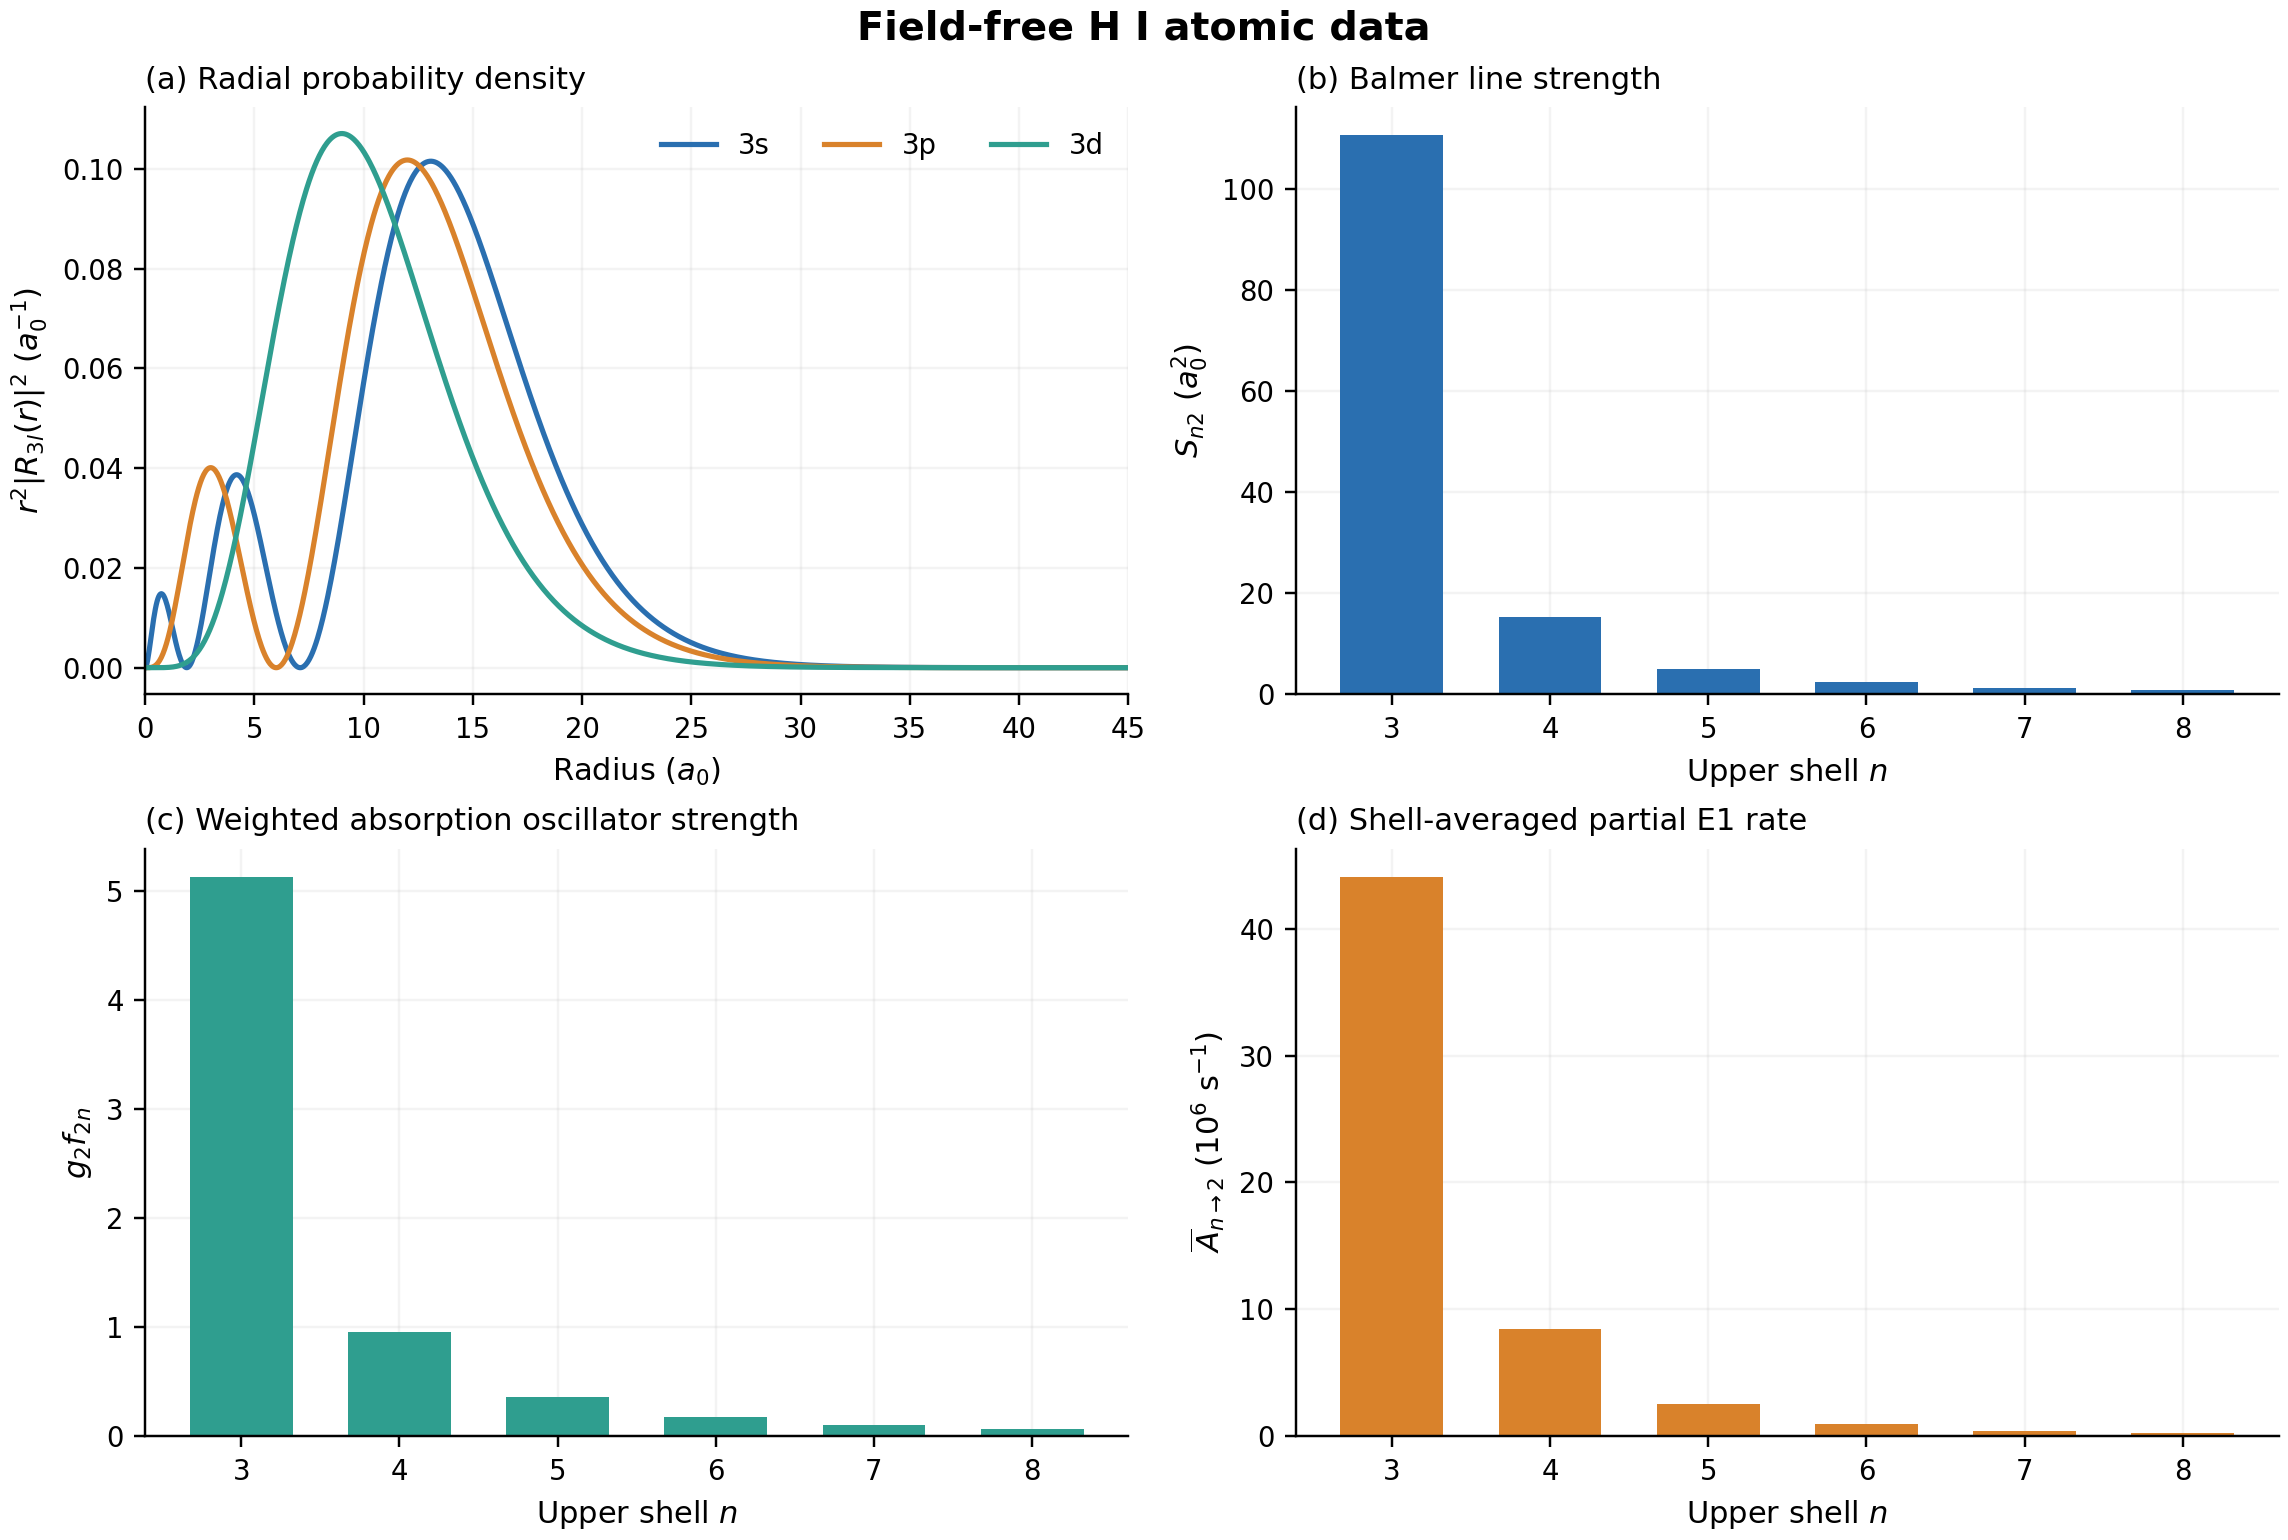
\includegraphics[width=\linewidth]{../docs/figures/examples/atomic_field_free.png}
\caption{Field-free hydrogen: (a) normalized $n=3$ radial probability
densities; (b) shell-summed Balmer line strengths; (c) weighted absorption
oscillator strengths; (d) E1 rates into $n=2$ averaged over each complete
upper shell. Only panel (d) requests $A=1$. Strengths contain no population
weights.}
\label{fig:atomic_field_free}
\end{figure}

A rate into one selected lower shell is partial, so its reciprocal is
generally not the upper-state lifetime. The function
\texttt{natural\_decay\_rates(n)} sums over every lower shell, but only
within E1 theory. Its zero rate for field-free hydrogen 2s does not imply an
infinite physical lifetime, since non-E1 processes are excluded.

\subsection{Fixed-Field Dressed Transitions and Radiative Rates}

A \texttt{LineProfile} object supplies its upper and lower shells, nuclear
charge, and isotope to convenient accessors. The radial accessors return
field-free quantities even when $B$ is nonzero.
\texttt{radial\_wavefunction} defaults to \texttt{shell='upper'}; select
\texttt{shell='lower'} for the lower shell. The
\texttt{field\_free\_einstein\_a\_s} property uses the object's isotope mass.

\begin{minipage}{\linewidth}
\lstinputlisting[language=Python,basicstyle=\footnotesize\ttfamily,
  columns=fullflexible,breaklines=true,showstringspaces=false,gobble=4,
  linerange={DRESSED_BEGIN-DRESSED_END},includerangemarker=false]
  {../examples/atomic_api_and_stark_maps.py}
\end{minipage}

\texttt{compute\_discrete} returns \texttt{self} and stores its result in
\texttt{lp.discrete}. The result includes photon energies
\texttt{energy\_ev}, detunings from the physical reference
\texttt{detuning\_ev}, and the corresponding \texttt{wavelength\_nm},
\texttt{frequency\_thz}, and \texttt{wavenumber\_cm}. Its
\texttt{strength} values are individual squared dipoles in $a_0^2$ without
population factors. The polarization label \texttt{q} is $0$ for $\pi$,
$-1$ for $\sigma^+$, and $+1$ for $\sigma^-$.

The lazily evaluated \texttt{einstein\_a\_s} property converts each retained
transition's field-shifted photon energy and squared dipole to an E1 rate:
\begin{equation}
 A_{pkq}=\frac{4\alpha^3}{3\tau_{\mathrm{au}}}
 \left(\frac{E_{pk}}{E_{\mathrm h}}\right)^3 S_q(p,k),
 \qquad \tau_{\mathrm{au}}=\frac{\hbar}{E_{\mathrm h}}.
\label{eq:atomic_api_einstein}
\end{equation}
Here $E_{\mathrm h}$ is the Hartree energy; the ratio uses matching energy
units and $S_q$ is the numerical squared dipole in $a_0^2$. Individual
resolved transitions require no additional degeneracy division.

The \texttt{upper\_partial\_decay\_rate\_s} property sums those rates by
\texttt{upper\_idx}, producing $2n_u^2$ values through \texttt{LineProfile}.
It includes only the selected lower shell and transitions retained by
\texttt{min\_strength}. Set \texttt{min\_strength=0.0} to retain all nonzero
strengths when summing rates. Upper and lower indices refer to independently
energy-sorted eigensystems at the current field; they do not track a state
across field configurations.

\begin{figure}[H]
\centering
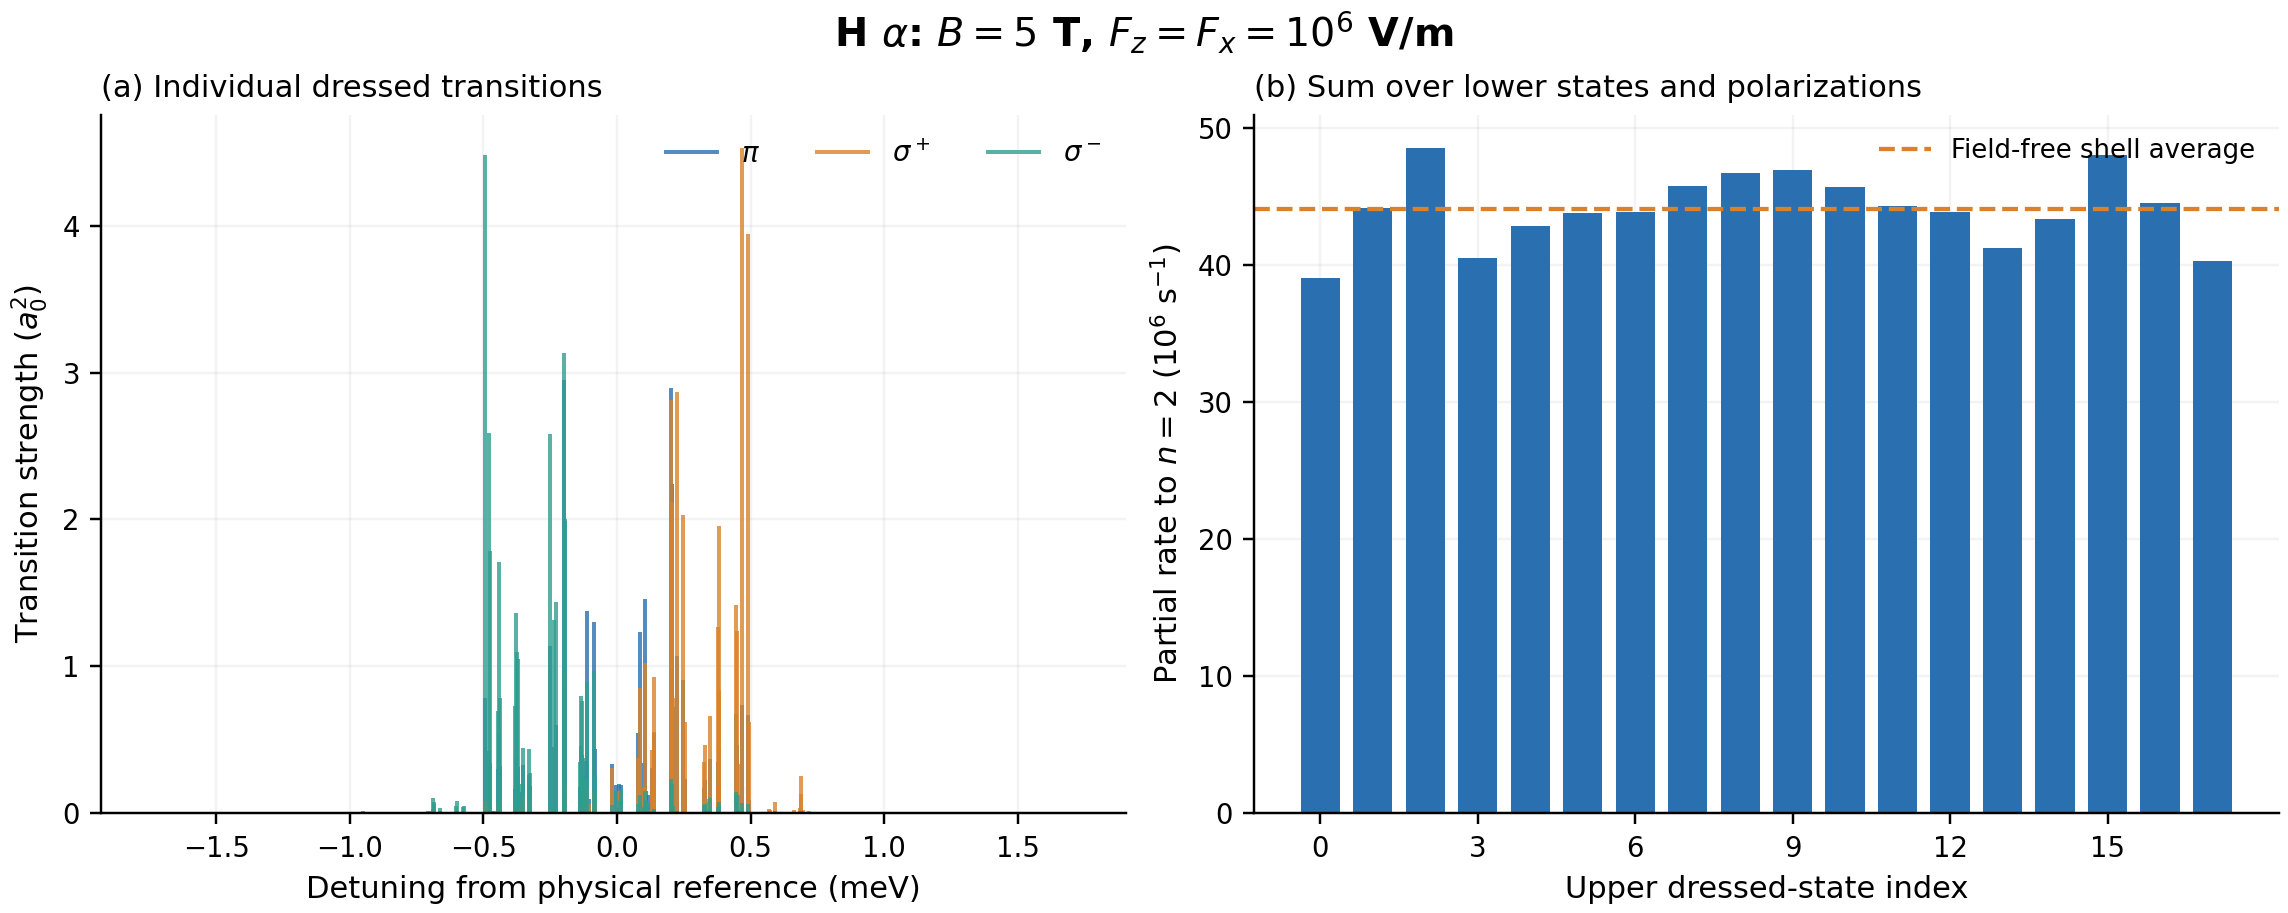
\includegraphics[width=\linewidth]{../docs/figures/examples/atomic_dressed_transitions.png}
\caption{H$\alpha$ at $B=5$ T and $F_z=F_x=10^6$ V/m, using empirical
hydrogen energies. Left: polarized transition strengths. Right: partial
rates into $n=2$ by upper dressed-state index; the dashed line is the
isotope-aware field-free shell average. Neither panel includes broadening,
population weights, or a plasma microfield average.}
\label{fig:atomic_dressed_transitions}
\end{figure}

The plasma density and temperature do not affect this fixed-field
calculation. Static, FFM, and discrete calls default to empirical H/D/T
energies; pass \texttt{use\_empirical\_data=False} to the calculation for
analytical energies, ions with $Z>1$, or shells beyond the bundled tables.

\subsection{Multi-Shell Stark Maps}

The separate \texttt{StarkMap} interface diagonalizes an analytical
hydrogenic Hamiltonian across a selected set of shells. It includes
inter-shell Stark coupling in that finite basis and does not change the
single-shell basis used by the production static and FFM profile solvers.
The map does not use the empirical H/D/T energy tables.

\begin{minipage}{\linewidth}
\lstinputlisting[language=Python,basicstyle=\footnotesize\ttfamily,
  columns=fullflexible,breaklines=true,showstringspaces=false,gobble=4,
  linerange={STARK_MAP_BEGIN-STARK_MAP_END},includerangemarker=false]
  {../examples/atomic_api_and_stark_maps.py}
\end{minipage}

The input field magnitudes are finite, nonnegative values in V/m. The
\texttt{angle\_deg} argument is the angle between the electric and magnetic
fields. A target tuple gives $(n,l,j,m_j)$; for parallel or antiparallel
fields its $m_j$ automatically selects a conserved symmetry sector. For
crossed fields, omit \texttt{mj}, since different projections mix.
The optional \texttt{max\_l} limits retained orbital angular momenta;
its default includes every allowed $l$ in the selected shells.
The \texttt{quadratic\_zeeman} flag controls the diamagnetic term.
The legacy \texttt{fine\_structure=False} setting omits mass-velocity and
Darwin corrections while retaining spin-orbit coupling.

\begin{minipage}{\linewidth}
\begin{lstlisting}[language=Python,basicstyle=\footnotesize\ttfamily,
  columns=fullflexible,breaklines=true,showstringspaces=false]
result = maps[0]
fig, ax = result.plot(unit="GHz", reference="target_zero_field",
                      field_unit="V/cm")
ax.set_ylim(-500, 500)
\end{lstlisting}
\end{minipage}

\begin{figure}[H]
\centering
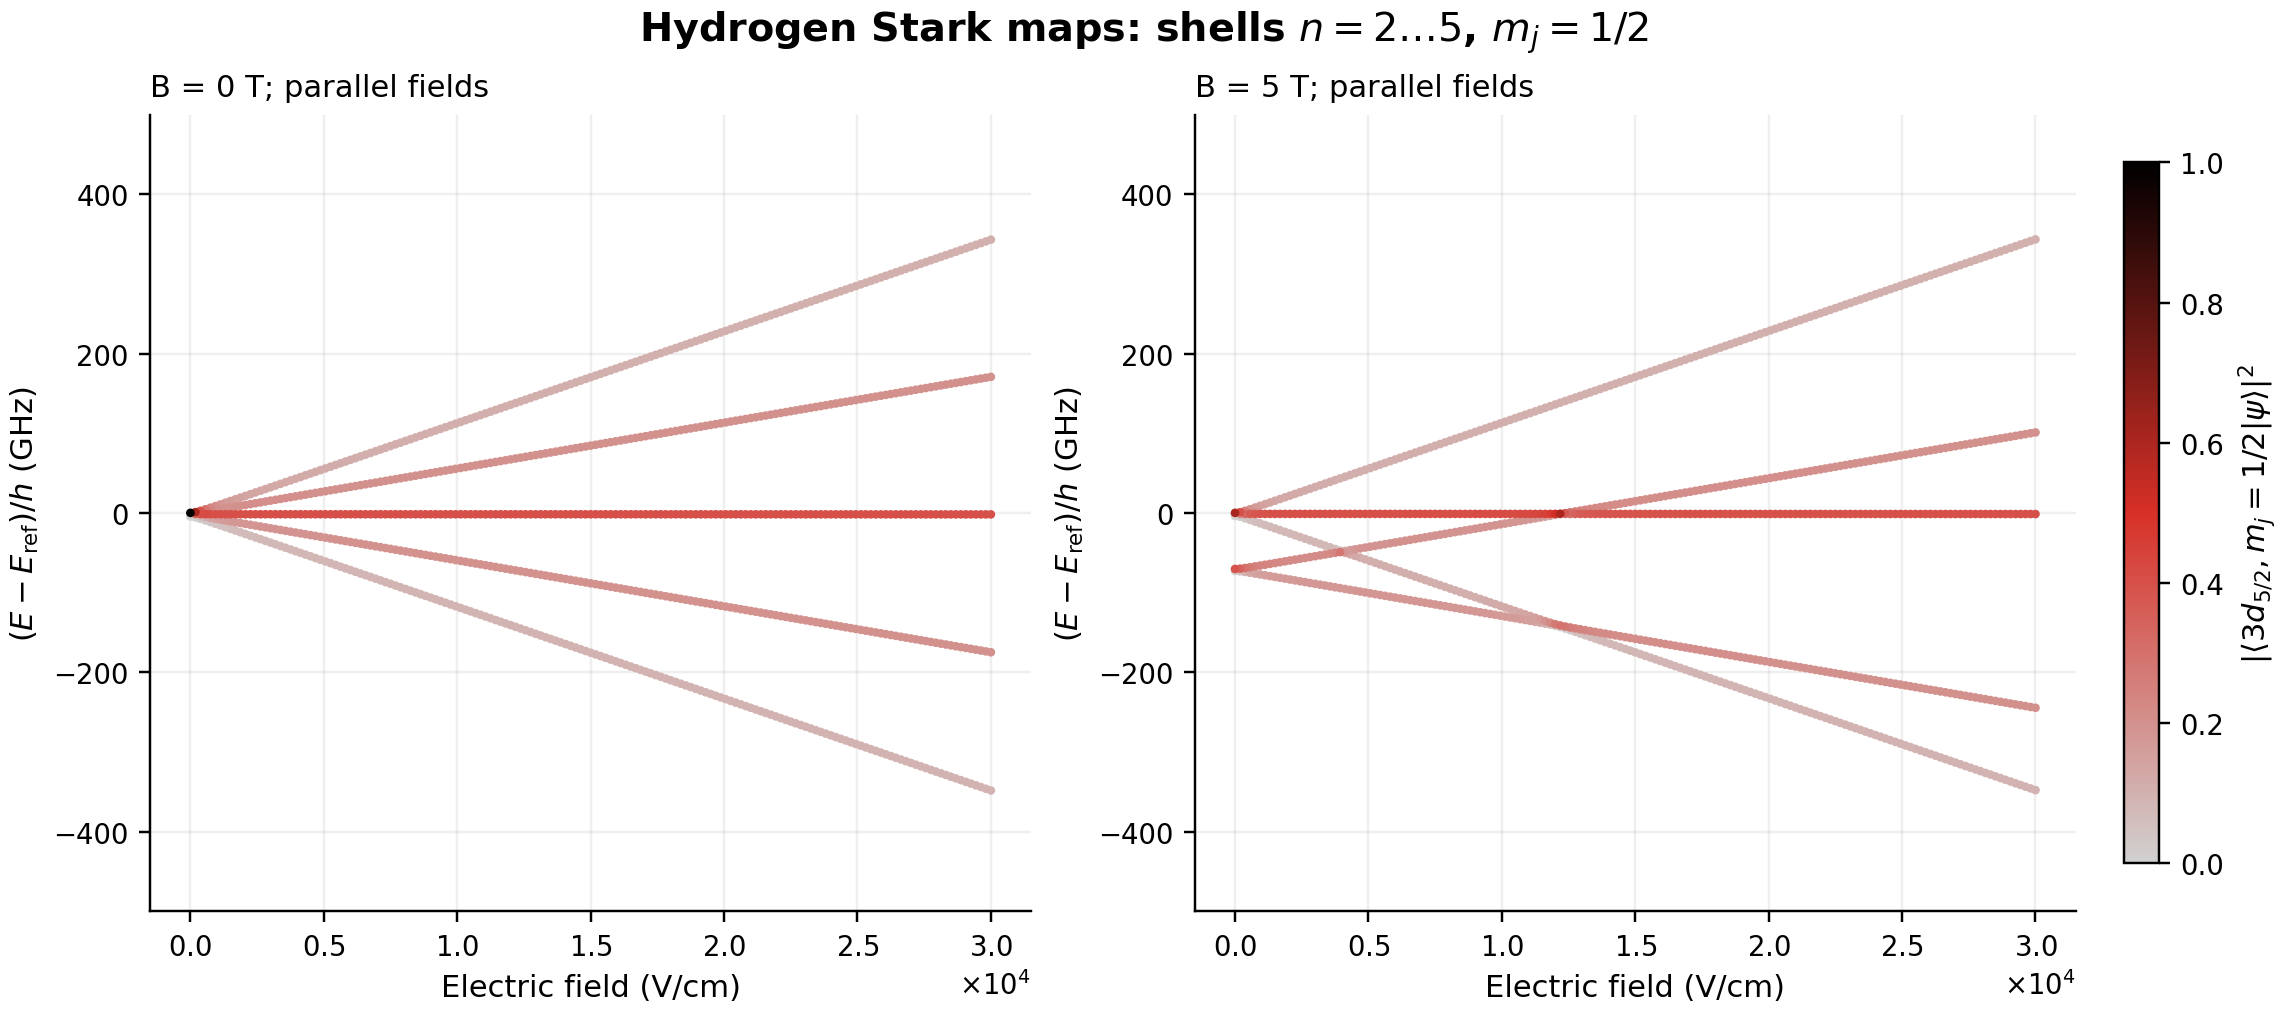
\includegraphics[width=\linewidth]{../docs/figures/examples/hydrogen_stark_map.png}
\caption{Hydrogen Stark maps for shells $n=2,3,4,5$, restricted to
$m_j=1/2$. Color gives $|\langle3d_{5/2},m_j=1/2|\psi\rangle|^2$.
Each panel subtracts its own zero-electric-field reference at the stated
$B$. The displayed window is $\pm500$ GHz; all 24 selected states enter
each calculation. The maximum field is $3\times10^6$ V/m, or
$3\times10^4$ V/cm. These overlap weights are neither populations nor
line strengths.}
\label{fig:hydrogen_stark_map}
\end{figure}

The arrays \texttt{energies\_ev} and \texttt{highlights} have shape
\texttt{(number\_of\_fields,number\_of\_states)}. Energies are absolute
bound-state energies relative to ionization; highlights are squared target
overlaps. They sum to one at each field when a target is supplied and are
zero without a target. The \texttt{zero\_field\_energies\_ev} array is
calculated at zero electric field even if the sweep omits zero.

Use \texttt{shifted\_energies} for eV, meV, GHz, or cm$^{-1}$ output.
GHz means ordinary frequency $\Delta E/h$. The default reference
\texttt{target\_zero\_field} selects the zero-electric-field eigenstate
with the largest target overlap at the configured fixed $B$. Other choices
are \texttt{lowest\_zero\_field}, \texttt{ionization}, or a numeric
reference energy in eV. Without a target, explicitly choose one of these
other references for \texttt{plot} or \texttt{shifted\_energies}.
The plotting method returns \texttt{(fig,ax)} and accepts V/m or V/cm on
the horizontal axis.

The properties \texttt{dominant\_target\_indices} and
\texttt{dominant\_target\_energy\_ev} choose the largest instantaneous
overlap independently at each field. They can jump between branches and
do not perform adiabatic state tracking. Enlarge the retained shells and
any angular-momentum cutoff to check convergence for the field range and
energy shifts of interest. The finite basis and analytical energies limit
the physical accuracy of the map.
\endgroup
